% Chapter Overview

\chapter{Overview} % Main chapter title

\label{overview} % For referencing the chapter elsewhere, use \ref{overview}
This chapter describes the components of our Accountable and Private Network Architecture (APNA), starting with the roles of the ASes (Section \ref{sec:role_as}), followed by the use of ephemeral identifiers (Section\ref{sec:ephid}) and ending with an end-to-end communication example (Section \ref{sec:comm})

\section{Role of ASes} \label{sec:role_as}
In APNA, ASes play a very important role due to their strategic location inside the network. They act both as accountability agents and as privacy brokers. In order to act as \textit{accountability agents} you must know the identity of the host and since ASes already know the physical attachment point of their customers and thus they know their identities. Hence, ASes are the perfect candidates for  \textit{accountability agents} 

At the same time, ASes can protect the identity of their customers from all the other entities on the network by masking it out. Thus it acts as \textit{host privacy brokers}. In addition, ASes certify their customer-related information (e.g. public keys), which is then used to generate keys for pervasive data encryption at the network layer; thus ASes act as \textit{data-privacy brokers}.

\subsection{Accountability Functions}
As an \textit{accountability agent}, the AS performs the following functions.

\begin{itemize}
    \item  AS creates a strong notion of host identity. In other words, the AS needs to ensure that host cannot use multiple unauthorized identities for the communication. Since AS already authenticates their customers and are thus selected as accountability agents.
    \item AS creates a link between host identity and packet sent by the host. To this end, AS can either store every packet or insert a cryptographic mark into every packet. Since all the packets which a host sends, regardless of implementation it will go through the AS as it will be on the forwarding path. Therefore it is selected to establish this link. Using any other third party, which is not on the forwarding path will require some special mechanisms to forward all the packets to this service while on other hand its kind of natural for AS because of its strategic location in the network.
    \item Malicious traffic can be easily stopped by the AS. Thus, AS realizes the shutoff functionality by accepting and validating shutoff requests and blocking the corresponding flows. Since AS usually include exit nodes thus they can easily block the malicious traffic before it even reaches on the network.
\end{itemize}

\subsection{Privacy Functions} As \textit{privacy broker} AS performs the following functions.

\begin{itemize}
    \item In order to provide the ability the ability for a sender to hide its network address so it can hide its identity from the third party observes in the source domain, from transit ISPs and from the destination. The AS issues an Ephemeral IDentifier (EphID) that a host can use to mask his identity and use it as a source address. This identifier serves as a privacy preserving return address and thus not break bidirectional communication. However, EphIDs must be bound to a host identity and since ASes already know their identities they are well suited to perform this binding and act as \textit{host-privacy brokers}. We provide more details about EphIDs in the following section.
    \item AS also act as a certificate issuer, certifying that a public key indeed belongs to a host in the AS's network. More specifically the AS can vouch for the binding between an EphID that is issued to host and a public key that is bound to the identifier. Hence the AS becomes a \textit{data-privacy brokers} without revealing the identity of its customers.
\end{itemize}

\section{Ephemeral IDs} \label{sec:ephid}
The main idea behind our proposal is the use of ephemeral identifiers instead of IPv4/IPv6 addresses. EphIDs are unique identifiers associated with host identity at the same respecting their privacy by not leaking identity information. Since ASes are already aware about the identities of their customers, issuing EphIDs to their connected hosts enables the hosts to hide their identity without comprising accountability.

\subsection{EphID as an Accountability Unit}
EphIDs are like authorization tokens issued by AS to its customer. These tokens can be used for communication with other host on the internet. In order to issue these tokens strong host authentication is required: the host must prove its identity to the AS, and only then EphIDs can be issued.
\subsubsection{What is a valid host identifier?} 
The only requirement for Host Identifier (HID) is that it must represent a unique host within the AS boundary. For example, a HID could be a hash of the host's public key or a number that is assigned by the AS to the host (e.g., IPv4/IPv6 address). Hence there is no specific requirement how an AS assigns HIDs until unless its a uniquely identifies a host within that AS.
\\ \\
There can be multiple EphIDs that are associated with an HID, and the EphIDs are cryptographically bound to the HID such that only host's AS can determine that binding. Furthermore, an EphID serves as an accountability unit for shutoff requests. A shutoff request against an EphID terminates all flows of the host that use that EphID as the source identifier. In other words, flows with the same source EphID are \textit{fate-sharing} with respect to shutoff protocol. Blacklisting source EphIDs instead of source and destination EphID pair forces hosts to carefully manage its pool of assigned EphIDs.

\subsection{EphID as an Privacy Unit}
The EphID has two important roles as a privacy unit. It hides the identity of a host and provides a tool to achieve various notion of sender-X unlinkability (e.g., sender-flow unlinkability). An EphID is only meaningful to the issuing AS and opaque to all other parties. It reveals no information about host's identity to other hosts inside the same AS nor to the peer host that the host is communicating with.

EphIDs alone are insufficient for routing packets to a destination since EphID are meaningless outside the AS thus its impossible to route packets just on the basis of EphID. But SCION comes to rescue for that problem. Inside SCION intra-domain and inter-domain routing are handled separately. For inter-domain routing SCION uses \texttt{ISD-AS} number thus \texttt{(ISD-AS:EphID)} becomes a routable entity. Hence, the only leaked information is the \texttt{ISD-AS} where the host resides; the host's anonymity set becomes the size of the AS in terms of number of hosts.

\section{Communication Example} \label{sec:comm}
In this section we provide a high level idea about communication workflow inside APNA. The protocol description is provided in the following section. This section mainly describes all the important services that needs to be running inside AS for APNA to work.

AS needs to provide following functionality like issuing and manage EphIDs; authenticate the packets that its host send; and provide DNS Service for hostname resolution. For these tasks, the following logical entities are present in every AS.

\begin{figure}[th!!]
\centering
\noindent
\makebox[\textwidth]{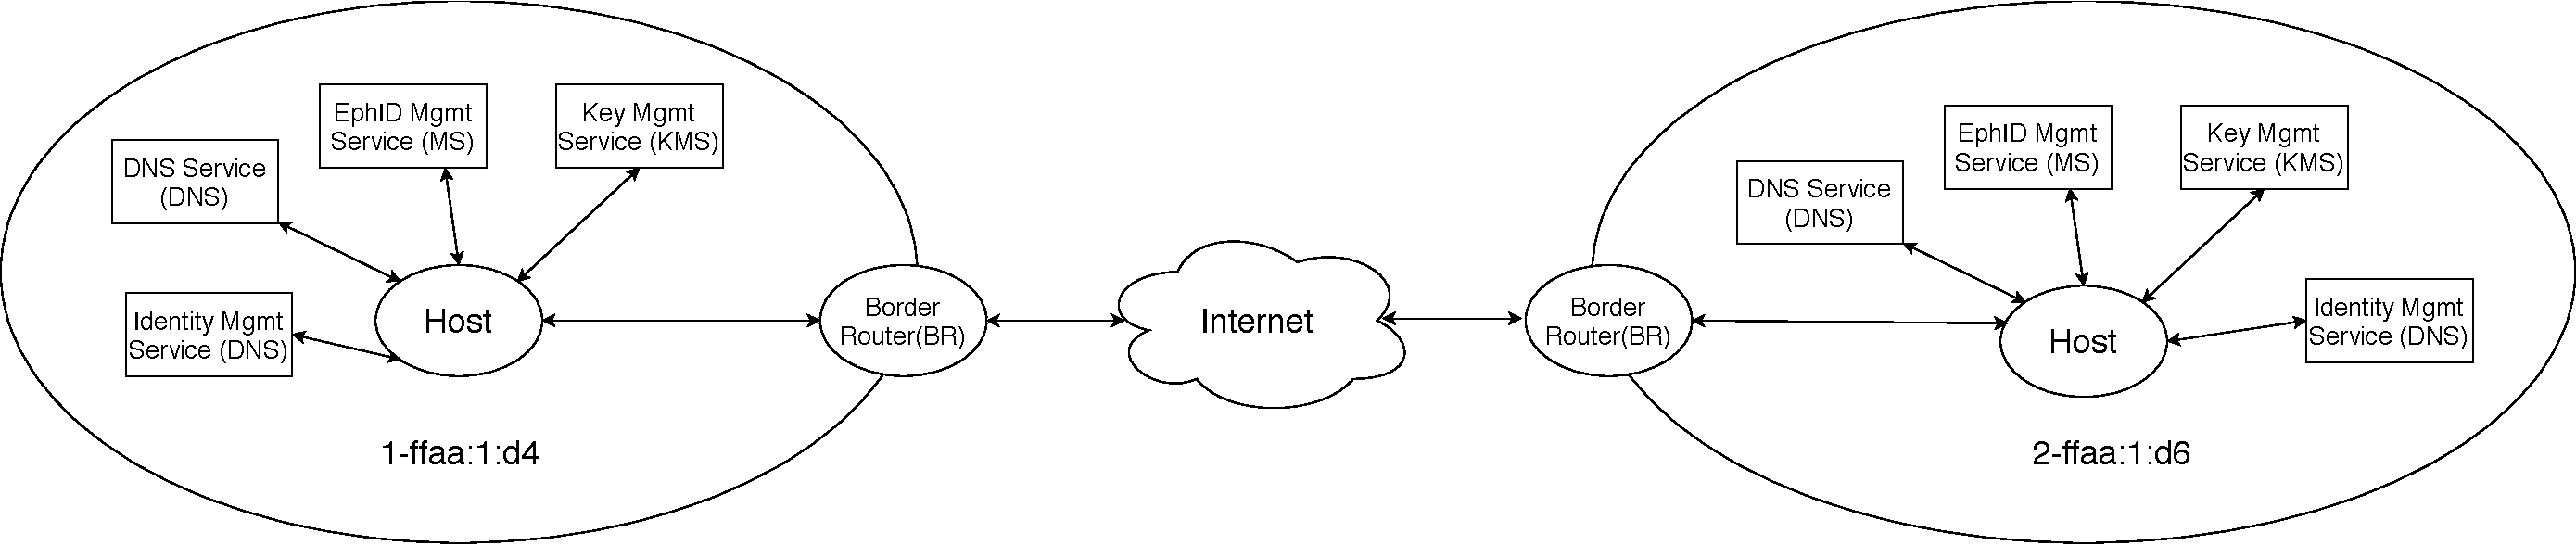
\includegraphics[scale=0.4]{Figures/end_to_end_comm.pdf}}
\decoRule
\caption[APNA End-to-end communication]{An end-to-end communication example}
\label{fig:end_to_end_comm_apna}
\end{figure}

\begin{itemize}
    \item \textbf{EphID Mgmt Service}: issues EphID to the host. (Refer Section \ref{sec:apna_ms})
    \item \textbf{DNS Service}: handle DNS related queries like Domain Registration, Domain Resolution etc. (Refer Section \ref{sec:apna_dns})
    \item \textbf{Identity Mgmt Service}: handles Host Identifier related queries for example converting IPv4/IPv6 address to HID and vice-versa (Refer Section \ref{sec:ims})
    \item \textbf{Key Mgmt Service}: authenticates and bootstraps hosts in the AS. (Refer Section \ref{sec:kms})
    \item \textbf{Border Router}: handles incoming and outgoing packets based on the \texttt{ISD-AS:EphID} tuple.
\end{itemize}

In Figure \ref{fig:end_to_end_comm_apna}, a host in \texttt{ISD-AS(1-ffaa:1:d4)} initiates a communication with host in \texttt{ISD-AS(2-ffaa:1:d6)}. Communication proceeds as described below:

\begin{itemize}
    \item \textbf{Host Bootstrapping:} the host authenticates to the KMS of its AS and registers it's shared secret with the AS and receives the bootstrapping information.
    \item \textbf{EphID Issuance}: the host contacts the EphID Mgmt Service of its AS to obtain an EphID.
    \item \textbf{DNS Operation}: the host either registers its domain name with the DNS service of its AS or the host queries for EphID of the registered domain name.
    \item \textbf{Data communication}: the host proceed with data communication using its \texttt{ISD-AS:EphID} tuple and their peers \texttt{ISD-AS:EphID} tuple which they obtain through DNS Service. If host want to encrypt their communication, they perform a connection establishment prior to the actual communication, to negotiate a shared key that will be used to encrypt their data packets. The shared key is derived from public keys that are associated with the EphIDs.
\end{itemize}

\section{APNA Protocol Details}
The main objective that we had in mind while designing APNA that it should be lightweight and efficient architecture and due to that following design choices were made:

\begin{itemize}
    \item Use of symmetric encryption heavily as compared to asymmetric encryption for example:
    \begin{itemize}
        \item In order to link EphIDs with HIDs symmetric encryption is used; this allows EphID Mgmt Service to efficiently obtain EphID from HID and vice-versa without using a mapping table, which can be large.
        \item Forwarding devices while verifying packet authenticity only perform symmetric cryptography, guaranteeing high forwarding performance.
    \end{itemize}
    \item Proof of sending the packet is embedded inside the packet, avoiding large amounts of stored state as ASes. 
\end{itemize}

\subsection{Assumptions}

\begin{itemize}
    \item We assume that the cryptographic primitive we use are secure. For instance we assume that authenticated encryption used for encrypting data communication is safe against chosen-ciphertext attacks (i.e., CCA-secure). We also require that EphID generation process is also CCA-secure and in future chapters we would describe an efficient CCA-secure encryption scheme to generate EphID.
    \item Every AS has a public key and a corresponding certificate; and there is a public-key infrastructure (e.g., RPKI) from which entity can retrive and verify AS-certificate. Fortunately inside SCION we have Certificate Server (\ref{sec:cert_server}) which contains AS level certificates provides the whole public key infrastructure.
    \item Hosts do not use connection sharing devices (e.g. NAT)
\end{itemize}
\newpage
\bgroup
\def\arraystretch{1.5}%
\begin{center}
\captionof{table}{Notation} \label{tab:notation} 
\begin{tabular}{r  l}
  \hline			
  $k_{A_{i}}$ & Symmetric key of $AS_i$ that is known among the infrastructure (e.g., routers, IMS, KMS)\\
  $k_{H_{i}A_{i}}$ & Symmetric key shared between host $H_i$ and its AS ($AS_i$) \\
  $K_{E_{i}E_{j}}$ & Symmetric key generated for the EphID pair $E_i$ and $E_j$ \\ 
  $HID_i$ & Host identifier (HID) assigned to host $H_i$ \\
  $EphID_h$ & An EphID issued to host $H$ \\
  $C_{EphID_{i}}$ & Certificate for EphID $EphID_i$ \\
  $K^{+}_{E}$, $K^{-}_{E}$ & Public, private key of entity E for both DH Exchange and Digital Signatures.\\
  $MAC_k(M)$ & Message M and MAC of M using symmetric key $k$ \\
  ${M}_{K^{-}}$ & Message M and Signature of M using private-key $K^{-}$ \\
  $E_{k}(M)$ & Symmetric encryption of M with key $k$. \\
  $E^{-1}_{k}(C)$ & Symmetric decryption of C with key $k$ \\
  \hline  
\end{tabular}
\end{center}
\egroup

\subsection{Host Bootstrapping}
A host authenticates to its AS using a well-established authentication protocol. For example, when a user subscribes to an Internet service provider, the provider creates the authentication credentials, and these credentials are preconfigured into an Internet access device (e.g., cable or DSL modem). The device performs the authentication protocol when the user connects it to the network.

The host (or his access device) creates a symmetric key $k_{HA}$ which serves multiple purpose. For example encrypting EphID request and reply message (refer Sec \ref{sec:why_encrypt}) and authenticating every packet that the host sends to the network. During authentication host securely sends $k_{HA}$ to the Key Management Service (KMS) by encrypting it using AS's public key ($K^{+}_{AS}$). 

Once the host is successfully authenticated, KMS of the AS performs the bootstrapping. During this procedure KMS creates a control EphID ($EphID_{h}^{ctrl}$) for the host which is later required for communicating with EphID Mgmt. Service or registering domain name with the DNS service. 

KMS stores the host information ($HID$, $k_{HA}$) and provides API for infrastructure entities to access in the AS e.g., Border Routers, EphID Mgmt. Service, Identity Mgmt. Service etc. The infrastructure will need this information in order to handle packets that are originating from and destined to this host. Specifically, the entities need to learn the HID of the host($HID$) and the shared key ($k_{HA}$) so that they can verify the authenticity of the packets that originate from the host.

Finally the KMS returns the control EphID ($EphID_{h}^{ctrl}$) with its expiration time ($ExpTime$)

\begin{figure}[th!!]
\centering
\noindent
\makebox[\textwidth]{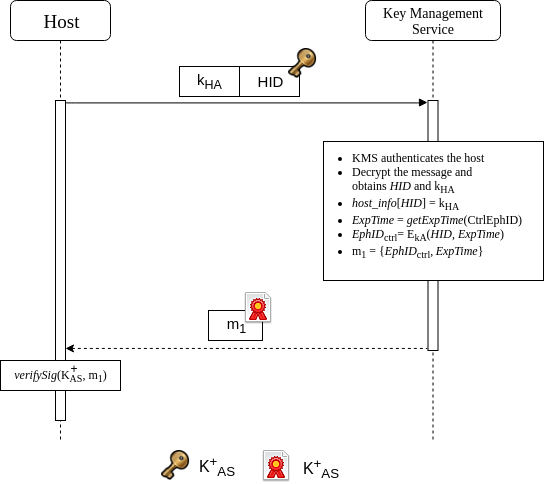
\includegraphics[scale=0.6]{Figures/kms.png}}
\decoRule
\caption[Host Bootstrapping]{Host bootstrapping with Key Management Service}
\label{fig:perf_dns}
\end{figure}

\subsection{Ephemeral ID Issuance}
An EphID is an encrypted token using the AS's secret key ($k_A$). It contains the host's $HID$ and expiration time that indicates the validity period for the EphID. One important point to note is that use of encryption instead of huge mapping tables enables issuing of EphID in a stateless fashion.

Each EphID is associated with a public/private key pair ($K^{+}_{EphID}$, $K^{-}_{EphID}$) which serves three purposes.
\begin{itemize}
    \item Mutual authentication with the peer host
    \item Help in Diffie-Hellman Key Exchange for obtaining the shared key with the peer host for data encryption
    \item Authenticate shutoff requests
\end{itemize}

To keep the data encryption key secret from AS, the host (not the AS) generates the key pair, and the private key is never revealed to the AS. The AS certifies the binding between an EphID and a public/private key pair by issuing a certificate ($C_{EphID}$) that has the same expiration time as the EphID. From the certificate, a peer host learns the public key ($K^{+}_{EphID}$) that is associated to the EphID as well as the EphID expiration time.

\subsection{Data Communication - APNA Session Key Derivation}
In this section, we will discuss about how hosts encrypt their communication and how APNA border routers forward the data packets.

\subsubsection{Data Communication with Network-Layer Encryption}
In order to encrypt the communication between hosts, they need to agree on shared symmetric key which would be used to encrypt the whole communication session. In order to derive this shared symmetric key hosts will perform Diffie-Hellman Key exchange. Note that two hosts can create multiple communication sessions and each session has a different symmetric key to ensure that disclosure of one encryption key does not compromise data privacy of other communication sessions.

Consider two hosts, A and B with EphIDs 